\documentclass[10pt]{article}
\usepackage[usenames]{color} %used for font color
\usepackage{amssymb} %maths
\usepackage{amsmath} %maths
\usepackage[utf8]{inputenc} %useful to type directly diacritic characters
\usepackage{tikz-feynman}\begin{document}
\textbf{\textcolor{blue}{Scattering amplitudes}}

A \textcolor{red}{scattering amplitude} is given in a diagrammatic form $\to$ \textcolor{red}{Feynman diagrams}:
\begin{eqnarray}
\nonumber
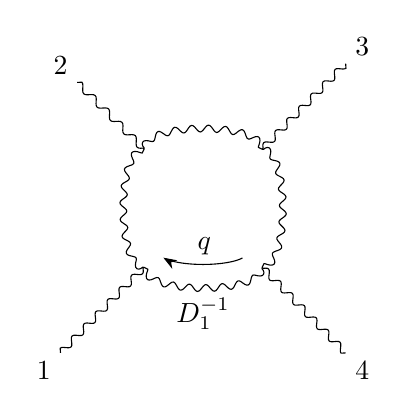
\begin{tikzpicture}
\begin{feynman}
  \vertex (k2) {2};
  \vertex [below right=of k2] (c);
  \vertex [right=of c] (d);
  \vertex [above right=of d] (k3) {3};
  \vertex [below=of c] (b);
  \vertex [right=of b] (a);
  \vertex [below left = of b] (k1) {1};
  \vertex [below right = of a] (k4) {4};
  
  \diagram* {
    (a) -- [boson] (k4),
    (b) -- [boson] (k1),
    (c) -- [boson] (k2),
    (d) -- [boson] (k3),
    (a) -- [boson, half left, looseness=0.6, momentum'=\(q\), edge label=\(D_1^{-1}\)] (b),
    (b) -- [boson, half left, looseness=0.6] (c),
    (c) -- [boson, half left, looseness=0.6] (d),
    (d) -- [boson, half left, looseness=0.6] (a),
  };
\end{feynman}
\end{tikzpicture}
\end{eqnarray}
This diagram represents a 1 loop, $(2\to 2)$ scattering process.
We translate this kind of diagram into momentum integral form $\to$ a \textcolor{red}{scattering amplitude}.
\begin{eqnarray}
\nonumber
%\int d^dq \mathcal{A}(q) = 
\int d^dq \frac{N(q)}{D_1 D_2 D_3 D_4}
\end{eqnarray}
where $N(q)$ is determined by the theoretical model, e.g., the Standard Model.

\end{document}